% some changes 

\documentclass{exam}

\usepackage{fullpage}
\usepackage{enumerate}
\usepackage{siunitx} 
\usepackage{graphicx}
\usepackage[fleqn]{amsmath}
\usepackage{cancel}
\usepackage{polynom}
\usepackage{float}
\usepackage{mdwlist}
\usepackage{booktabs}
\usepackage{cancel}
\usepackage{polynom}
\usepackage{caption}

\newcommand{\degree}{\ensuremath{^\circ}} 
\everymath{\displaystyle}

% \begin{figure}[H]
%   \centering
%   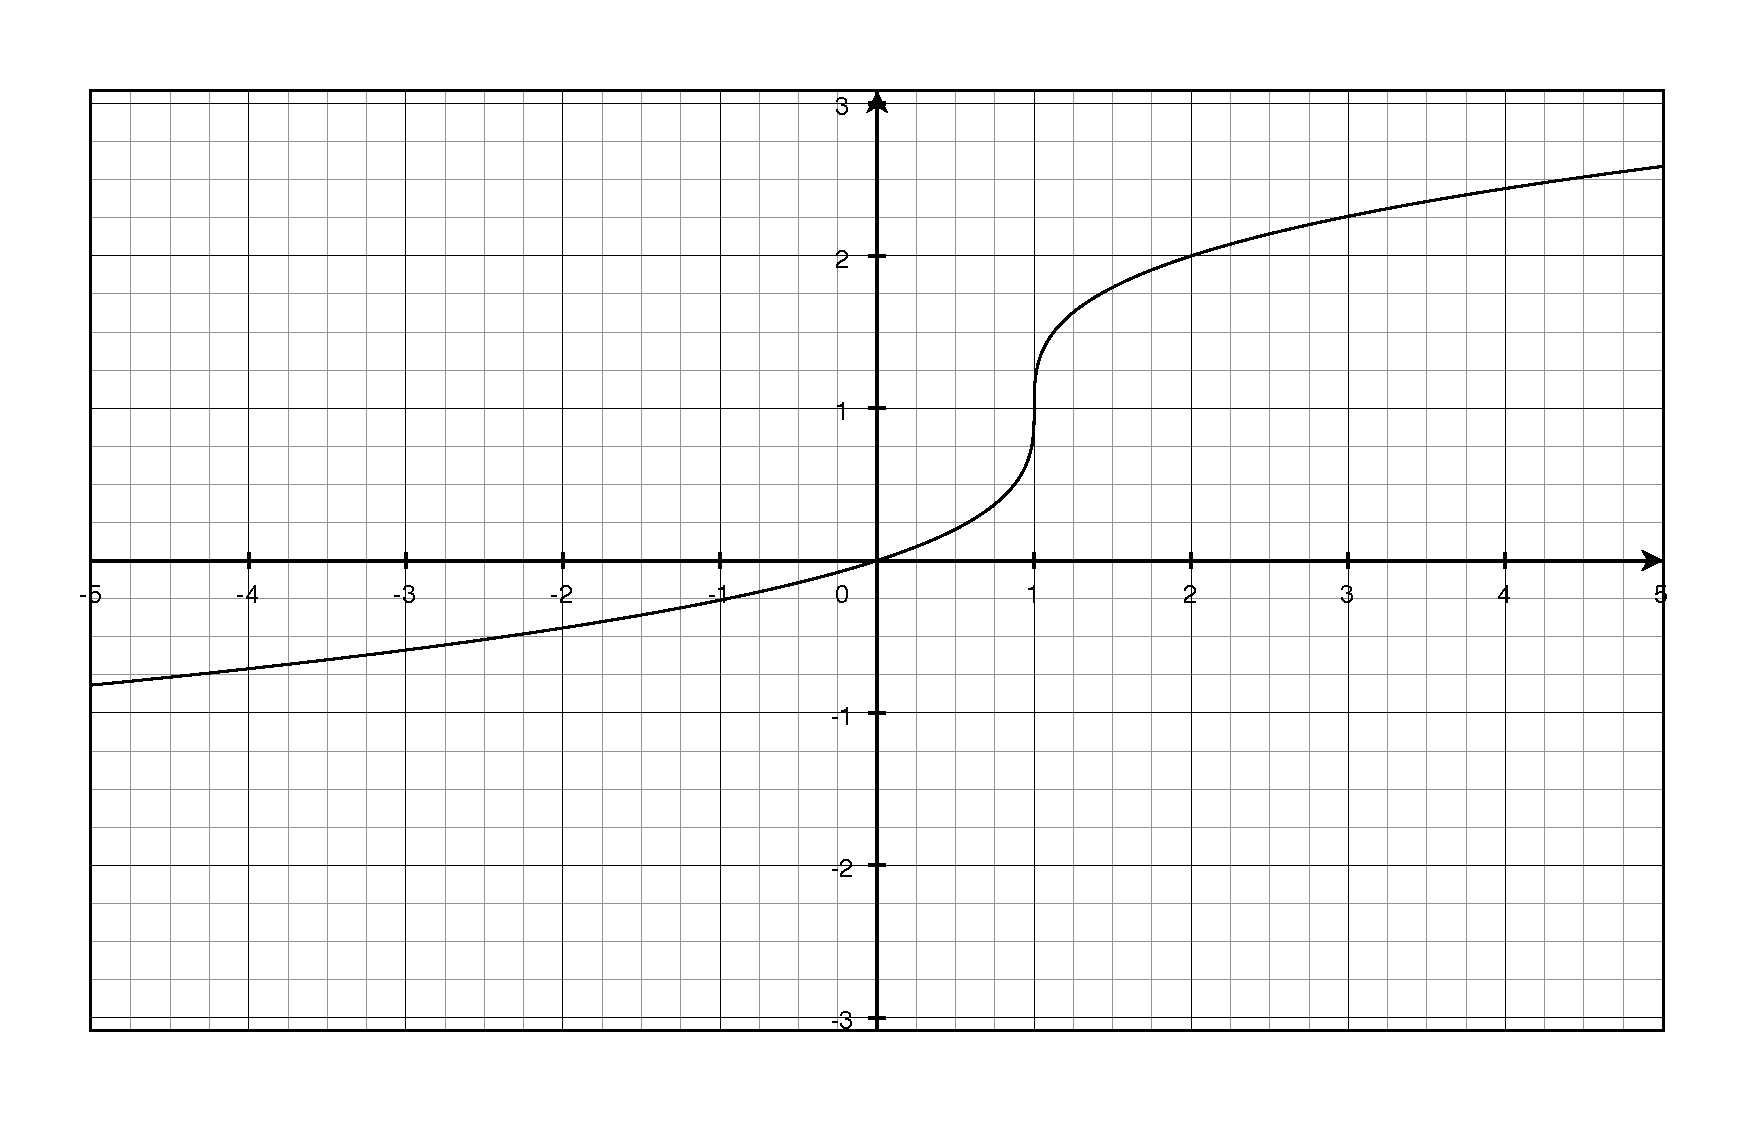
\includegraphics[scale=.3]{question7.eps}
%   \caption*{Question 7}
% \end{figure}

% \begin{tabular}{cc}
% \toprule
% period & amplitude \\
% \midrule
%   $\pi$ & $2$ \\
% \bottomrule
% \end{tabular}

% \textwidth 6.5 in

\printanswers

\ifprintanswers 
\usepackage{2in1, lscape} 
\fi

\title{Math 263a \\ Homework Five}
\date{February 22, 2012}

\begin{document}

\maketitle

\section{Homework}

\begin{itemize*}
  \item Read Sections 2.7 and 3.1-3.2
  \item pp 91-93: 4-8, 12-15, 18-19, 30-33, 
  \item pp 104-106: 9-10, 12, 15-16, 18, 21
  \item pp 111-112: 5-8, 13-14, 19-20, 23-24
\end{itemize*}

\section{Extra Credit}
Page 92, problems 43 and 44

\ifprintanswers
\begin{description}
\item[43]
As suggested in the hint, we can define $g(x) = x - f(x)$.  

Since $f(x)$ is between $0$ and $1$, 
\begin{align*}
  -1 &\leq g(0) \leq 0 \\
  0  &\leq g(1) \leq 1  \\
\end{align*}

Let's look at the end points first:
\begin{itemize*}
\item If $g(0) = 0$ then $f(0) = 0$ and we've found that 0 works and we're done.
\item If $g(1) = 0$ then $f(1) = 1$ and we've found that 1 works and we're done.
\end{itemize*}

If we assume that either $g(0) \neq 0$ or $g(1) \neq 0$ then one of them is negative and the other one is positive and 0
is a number between $g(0)$ and $g(1)$.  From the {\em Intermediate Value Theorem}, there must be some $c$ in the range
$[0, 1]$ where $g(c) = 0$.  

For $c$:
\begin{align*}
  g(c)     &= 0 \\
  c - f(c) &= 0 \\
  f(c)     &= c \\
\end{align*}

\item[44]

The two interesting points are $x = 1$ and $x = 2$, since this is when a different equation takes effect.  

For the function to be continuous, the limit at $x = 1$ must the the same coming from either direction:
\begin{align*}
  \lim_{x \to 1} ax + b &= \lim_{x \to 1} x + 1 \\
  a + b &= 2 \\
\end{align*}
The limit at $x = 2$ also must the the same coming from either direction:
\begin{align*}
  \lim_{x \to 2} ax + b &= \lim_{x \to 2} 3x \\
  2a + b &= 6 \\
\end{align*}
Now we have two equations and two unknowns, so we can solve for $a$ and $b$, finding:
\begin{align*}
  a &= 4 \\
  b &= -2 \\
\end{align*}

\end{description}

\section{Section 2.7}
\begin{description}
\item[4]
Not continuous because 3 is not in the domain of $f$.

\item[5]
Not continuous because 3 is not in the domain of $f$.

\item[6]
Not continuous because 3 is not in the domain of $f$.

\item[7]
Continuous.

\item[8]
Continuous.

\item[12]
Not continuous:
\begin{align*}
  r(3) &= 23 \\
  \lim_{t \to 3} r(t) &= 27 \\
\end{align*}

\item[13]
Continuous.

\item[14]
Continuous.

\item[15]
Not continuous.  $\lim_{x \to 3} f(x)$ is not defined:
\begin{align*}
  \lim_{x \to 3-} f(x) &= -5 \\
  \lim_{x \to 3+} f(x) &= -2 \\
\end{align*}

\item[18]
\[
  \lim_{x \to 7} \frac{x^2 - 49}{x-7} = \lim_{x \to 7} \frac{(x+7)(x-7)}{x-7} = \lim_{x \to 7} x+7 = 14
\]

So $f(7)$ should be 14 to make $f$ continuous.

\item[19]
\[
  \lim_{x \to 3} \frac{2x^2 - 18}{3-x} = \lim_{x \to 3} \frac{2(x+3)(x-3)}{-(x-3)} = \lim_{x \to 3} -2x - 6 = -12
\]

So $f(3)$ should be -12 to make $f$ continuous.

\item[30]
Continuous everywhere.

\item[31]
\begin{align*}
  4 - x^2 &\leq 0 \\
  x^2 &\geq 4 \\
  x &\leq -2 \text{ or } x \geq 2 \\
\end{align*}

$G$ is not defined when $x \leq -2 \text{ or } x \geq 2$ and continuous everywhere else.

\item[32]
\begin{align*}
  \lim_{x \to 0} f(x) &= 0 = f(0) \\
  \lim_{x \to 1} f(x) &= 1 = f(1) \\
\end{align*}
So $f$ is continuous at the transition points.  It is also continuous everywhere else, since it is defined by polynomial functions.

\item[33]
\begin{align*}
  \lim_{x \to 1^-} &= -1 \\
  \lim_{x \to 1^+} &= 1 \\
  \lim_{x \to 1^-} &\neq \lim_{x \to 1^+}  \\
\end{align*}
So the limit is not defined at 1 and $g(x)$ is not continuous at this point.  It is continuous everywhere else.

\end{description}

\section{Section 3.1}

\begin{description}

\item[9]
\begin{align*}
  \lim_{h \to 0} &\frac{f(x+h) - f(x)}{h} = \lim_{h \to 0} \frac{(x+h)^2 - 1 - (x^2 - 1)}{h} \\
  &= \lim_{h \to 0} \frac{x^2 + 2xh + h^2 - 1 - x^2 + 1}{h} \\
  &= \lim_{h \to 0} \frac{2xh + h^2}{h} \\
  &= \lim_{h \to 0} 2x + h \\
  &= 2x \\
\end{align*}

\begin{tabular}{lrrrrr}
\toprule
x     & -2 & -1 & 0 & 1 & 2 \\
slope & -4 & -2 & 0 & 2 & 4 \\
\bottomrule
\end{tabular}

\item[10]
\begin{align*}
  \lim_{h \to 0} &\frac{f(x+h) - f(x)}{h} = \lim_{h \to 0} \frac{(x+h)^3 - 3(x+h) - (x^3 - 3x)}{h} \\
  &= \lim_{h \to 0} \frac{x^3 + 3x^2h + 3xh^2 + h^3 - 3x - 3h - x^3 + 3x}{h} \\
  &= \lim_{h \to 0} \frac{3x^2h + 3xh^2 + h^3 - 3h }{h} \\
  &= \lim_{h \to 0} 3x^2 - 3 + 3xh + h^2 \\
  &= 3x^2 - 3 \\
\end{align*}

\begin{tabular}{lrrrrr}
\toprule
x     & -2 & -1 &  0 & 1 & 2 \\
slope &  9 &  0 & -3 & 0 & 9 \\
\bottomrule
\end{tabular}

\item[12]
First find an equation for the slope:
\begin{align*}
  \lim_{h \to 0} &\frac{f(x+h) - f(x)}{h} = \lim_{h \to 0} \frac{\cfrac{1}{x+h-1} - \cfrac{1}{x-1}}{h} \\
  &= \lim_{h \to 0} \frac{x - 1 - (x+h-1)}{h(x+h-1)(x-1)} \\
  &= \lim_{h \to 0} \frac{-h}{h(x+h-1)(x-1)} \\
  &= \lim_{h \to 0} \frac{-1}{(x+h-1)(x-1)} \\
  &= - \frac{1}{(x-1)^2} \\
\end{align*}
The slope at the point we're interested in is: $- \frac{1}{(0-1)^2} = -1$.

Now we have the slope, we can use the point $(0, -1)$ to find the equation of the tangent line:
\begin{align*}
  y - y_0 &= m(x - x_0) \\
  y + 1   &= -1(x - 0) \\
  y       &= -x - 1 \\
\end{align*}

\item[15]
First find an equation for the velocity:
\begin{align*}
  \lim_{h \to 0} &\frac{f(t+h) - f(t)}{h} = \lim_{h \to 0} \frac{\sqrt{2(t + h) + 1} - \sqrt{2t + 1}}{h} \\
  &= \lim_{h \to 0} \frac{\sqrt{2t + 2h + 1} - \sqrt{2t + 1}}{h} \left( \frac{\sqrt{2t + 2h + 1} + \sqrt{2t + 1}}{\sqrt{2t + 2h + 1} + \sqrt{2t + 1}} \right) \\
  &= \lim_{h \to 0} \frac{2t + 2h + 1 - 2t - 1}{h(\sqrt{2t + 2h + 1} + \sqrt{2t + 1})} \\
  &= \lim_{h \to 0} \frac{2}{\sqrt{2t + 2h + 1} + \sqrt{2t + 1}} \\
  &= \frac{1}{\sqrt{2t + 1}} \\
\end{align*}

\begin{enumerate}[a]
\item
The velocity at $t = \alpha$ is $v(\alpha) = \frac{1}{\sqrt{2\alpha + 1}}$

\item
\begin{align*}
  \frac{1}{2} &= \frac{1}{\sqrt{2t + 1}} \\
  \frac{1}{4} &= \frac{1}{2t + 1} \\
  2t + 1 &= 4 \\
  t &= \frac{3}{2} \\     
\end{align*}

\end{enumerate}

\item[16]

The velocity is:
\begin{align*}
  \lim_{h \to 0} &\frac{-(t+h)^2 + 4(t+h) - (-t^2 + 4t)}{h} \\
   &= \lim_{h \to 0} \frac{-(t^2 + 2ht + h^2) + 4t+ 4h + t^2 - 4t}{h} \\
   &= \lim_{h \to 0} \frac{-t^2 - 2ht - h^2 + 4t+ 4h + t^2 - 4t}{h} \\
   &= \lim_{h \to 0} \frac{ - 2ht - h^2 + 4h}{h} \\
   &= \lim_{h \to 0}  -2t - h + 4 \\
   &= -2t + 4 \\
\end{align*}

The velocity is zero when:
\begin{align*}
  -2t + 4 &= 0 \\
  2t &= 4 \\
  t &= 2 \\
\end{align*}

\pagebreak

\item[18]
\begin{enumerate}[a]

\item 
\[
  p(3) - p(2) = 9,000 - 4,000 = 5,000 \text{ dollars}
\]

\item
\[
  p_{average} = \frac{p(2.5) - p(2)}{0.5} = 4,500 \text{ dollars/year}
\]

\item
The equation for the instantaneous profit is:
\begin{align*}
  \lim_{h \to 0} &\frac{f(t+h) - f(t)}{h} = \lim_{h \to 0} \frac{1000(t + h)^2 - 1000t^2}{h} \\
  &= \lim_{h \to 0} \frac{1000(t^2 + 2th + h^2) - 1000t^2}{h} \\
  &= \lim_{h \to 0} 2000t + 2000h \\
  &= 2000t \text{ dollars/year} \\
\end{align*}

At $t = 2$, the rate of profit is $2000 \cdot 2 = 4000$ dollars/year.

\end{enumerate}

\item[21]
The equation for the acceleration is:
\begin{align*}
  \lim_{h \to 0} &\frac{f(t+h) - f(t)}{h} = \lim_{h \to 0} \frac{2(t + h)^2 - 2t^2}{h} \\
  &= \lim_{h \to 0} \frac{2(t^2 + 2th + h^2) - 2t^2}{h} \\
  &= \lim_{h \to 0} 4t + 2h \\
  &= 4t \\
\end{align*}

At $t = 1$, the acceleration is $4 \cdot 1 = 4$.

\end{description}

\section{Section 3.2}

\begin{description}
\item[5]
\begin{align*}
  \lim_{h \to 0} &\frac{f(t+h) - f(t)}{h} = \lim_{h \to 0} \frac{2(t + h) + 1 - (2t + 1)}{h} \\
  &= \lim_{h \to 0} \frac{2t + 2h + 1 - 2t - 1)}{h} \\
  &= \lim_{h \to 0} \frac{2h}{h} \\
  &= \lim_{h \to 0} 2 \\
  &= 2
\end{align*}

\item[6]
\begin{align*}
  \lim_{h \to 0} &\frac{f(t+h) - f(t)}{h} = \lim_{h \to 0} \frac{\alpha(t + h) + \beta - (\alpha t + \beta)}{h} \\
  &= \lim_{h \to 0} \frac{\alpha t + \alpha h + \beta - \alpha t - \beta)}{h} \\
  &= \lim_{h \to 0} \frac{\alpha h}{h} \\
  &= \lim_{h \to 0} \alpha  \\
  &= \alpha
\end{align*}

\item[7]
\begin{align*}
  \lim_{h \to 0} &\frac{f(x+h) - f(x)}{h} = \lim_{h \to 0} \frac{3(x + h)^2 + 4 - (3x^2 + 4)}{h} \\
  &= \lim_{h \to 0} \frac{3(x^2 + 2xh + h^2) + 4 - 3x^2 - 4}{h} \\
  &= \lim_{h \to 0} \frac{3x^2 + 6xh + 3h^2 - 3x^2}{h} \\
  &= \lim_{h \to 0} \frac{6xh + 3h^2}{h} \\
  &= \lim_{h \to 0} 6x + 3h \\
  &= 6x \\
\end{align*}

\item[8]
\begin{align*}
  \lim_{h \to 0} &\frac{f(x+h) - f(x)}{h} = \lim_{h \to 0} \frac{(x + h)^2 + x+h + 1 - (x^2 + x + 1)}{h} \\
  &= \lim_{h \to 0} \frac{x^2 + 2xh + h^2 + x+h + 1 - x^2 - x - 1}{h} \\
  &= \lim_{h \to 0} \frac{2xh + h + h^2}{h} \\
  &= \lim_{h \to 0} 2x + 1 + h \\
  &= 2x + 1 \\
\end{align*}

\item[13]
\begin{align*}
  \lim_{h \to 0} &\frac{f(x+h) - f(x)}{h} = \lim_{h \to 0} \frac{\cfrac{2}{x + h} - \cfrac{2}{x}}{h} \\
  &= \lim_{h \to 0} \frac{2x - 2x - 2h}{hx(x+h)} \\
  &= \lim_{h \to 0} \frac{-2}{x(x+h)} \\
  &= - \frac{2}{x^2} \\
\end{align*}

\item[14]
\begin{align*}
  \lim_{h \to 0} &\frac{f(x+h) - f(x)}{h} = \lim_{h \to 0} \frac{\cfrac{1}{x + h + 1} - \cfrac{1}{x + 1}}{h} \\
  &= \lim_{h \to 0} \frac{x + 1 - x - h - 1}{h(x+1)(x+h+1} \\
  &= \lim_{h \to 0} \frac{-h}{h(x+1)(x+h+1)} \\
  &= \lim_{h \to 0} \frac{-1}{(x+1)(x+h+1)} \\
  &= - \frac{1}{(x+1)^2} \\
\end{align*}

\item[19]
\begin{align*}
  \lim_{h \to 0} &\frac{f(x+h) - f(x)}{h} = \lim_{h \to 0} \frac{\sqrt{3x + 3h} - \sqrt{3x}}{h} \\
  &= \lim_{h \to 0} \frac{\sqrt{3x + 3h} - \sqrt{3x}}{h} \left( \frac{\sqrt{3x + 3h} + \sqrt{3x}}{\sqrt{3x + 3h} + \sqrt{3x}} \right) \\
  &= \lim_{h \to 0} \frac{3x + 3h - 3x}{h \left( \sqrt{3x + 3h} + \sqrt{3x} \right) } \\
  &= \lim_{h \to 0} \frac{3}{\sqrt{3x + 3h} + \sqrt{3x}} \\
  &= \frac{3}{2\sqrt{3x}} \\
\end{align*}

\item[20]
\begin{align*}
  \lim_{h \to 0} &\frac{f(x+h) - f(x)}{h} = \lim_{h \to 0} \frac{\cfrac{1}{\sqrt{3x + 3h}} - \cfrac{1}{\sqrt{3x}}}{h} \\
  &= \lim_{h \to 0} \frac{\sqrt{3x} - \sqrt{3x + 3h}}{h (\sqrt{3x})(\sqrt{3x + 3h})} \left( \frac{\sqrt{3x} + \sqrt{3x + 3h}}{\sqrt{3x} + \sqrt{3x + 3h}} \right) \\
  &= \lim_{h \to 0} \frac{3x - 3x - 3h}{h (\sqrt{3x})(\sqrt{3x + 3h})(\sqrt{3x} + \sqrt{3x + 3h})} \\
  &= \lim_{h \to 0} \frac{ -3}{(\sqrt{3x})(\sqrt{3x + 3h})(\sqrt{3x} + \sqrt{3x + 3h})} \\
  &= \frac{ -3}{3x(2\sqrt{3x})} \\
  &= \frac{ -1}{2x\sqrt{3x})} \\
\end{align*}

\item[23]
\begin{align*}
  \lim_{t \to x} &\frac{f(t) - f(x)}{t - x} = \lim_{t \to x} \frac{t^2 - 3t - (x^2 - 3x)}{t - x} \\
  &= \lim_{t \to x} \frac{t^2 - x^2 - 3t + 3x}{t - x} \\
  &= \lim_{t \to x} \frac{(t+x)(t-x) - 3(t-x)}{t - x} \\
  &= \lim_{t \to x} t+x - 3 \\
  &= 2x - 3 \\
\end{align*}

\item[24]
\begin{align*}
  \lim_{t \to x} &\frac{f(t) - f(x)}{t - x} = \lim_{t \to x} \frac{t^3 + 5t - (x^3 + 5x)}{t - x} \\
  &= \lim_{t \to x} \frac{t^3 - x^3 + 5t - 5x}{t - x} \\
  &= \lim_{t \to x} \frac{(t-x)(t^2 + tx + x^2) + 5(t - x))}{t - x} \\
  &= \lim_{t \to x} t^2 + tx + x^2 + 5 \\
  &= 3x^2 + 5 \\
\end{align*}

\end{description}

\else

\vspace{10 cm}

% {\em People like us, who believe in physics, know that the distinction between past, present, and future is only a
%   stubbornly persistent illusion.}
{\em Unthinking respect for authority is the greatest enemy of truth.}

\vspace{.2 cm}

\hspace{1 cm} --Albert Einstein

\fi

\end{document}

